% %%%%%%%%%%%%%%%%%%%%%%%%%%%%%%%%%%%%%%%%%%%%%%%%%%%%%%%%%%%%%%%%% SECTION FIVE
% %%%%%%%%%%%%%%%%%%%%%%%%%%%%%%%%%%%%%%%%%%%%%%%%%%%%%%%%%%%%%%%%%%%%%%%%%%%%%%
\section{Stereo Pairs}

\subsection{Coincidenti}

\begin{figure*}[t]
    \centering
    \begin{subfigure}[t]{0.99\textwidth}
        \centering
        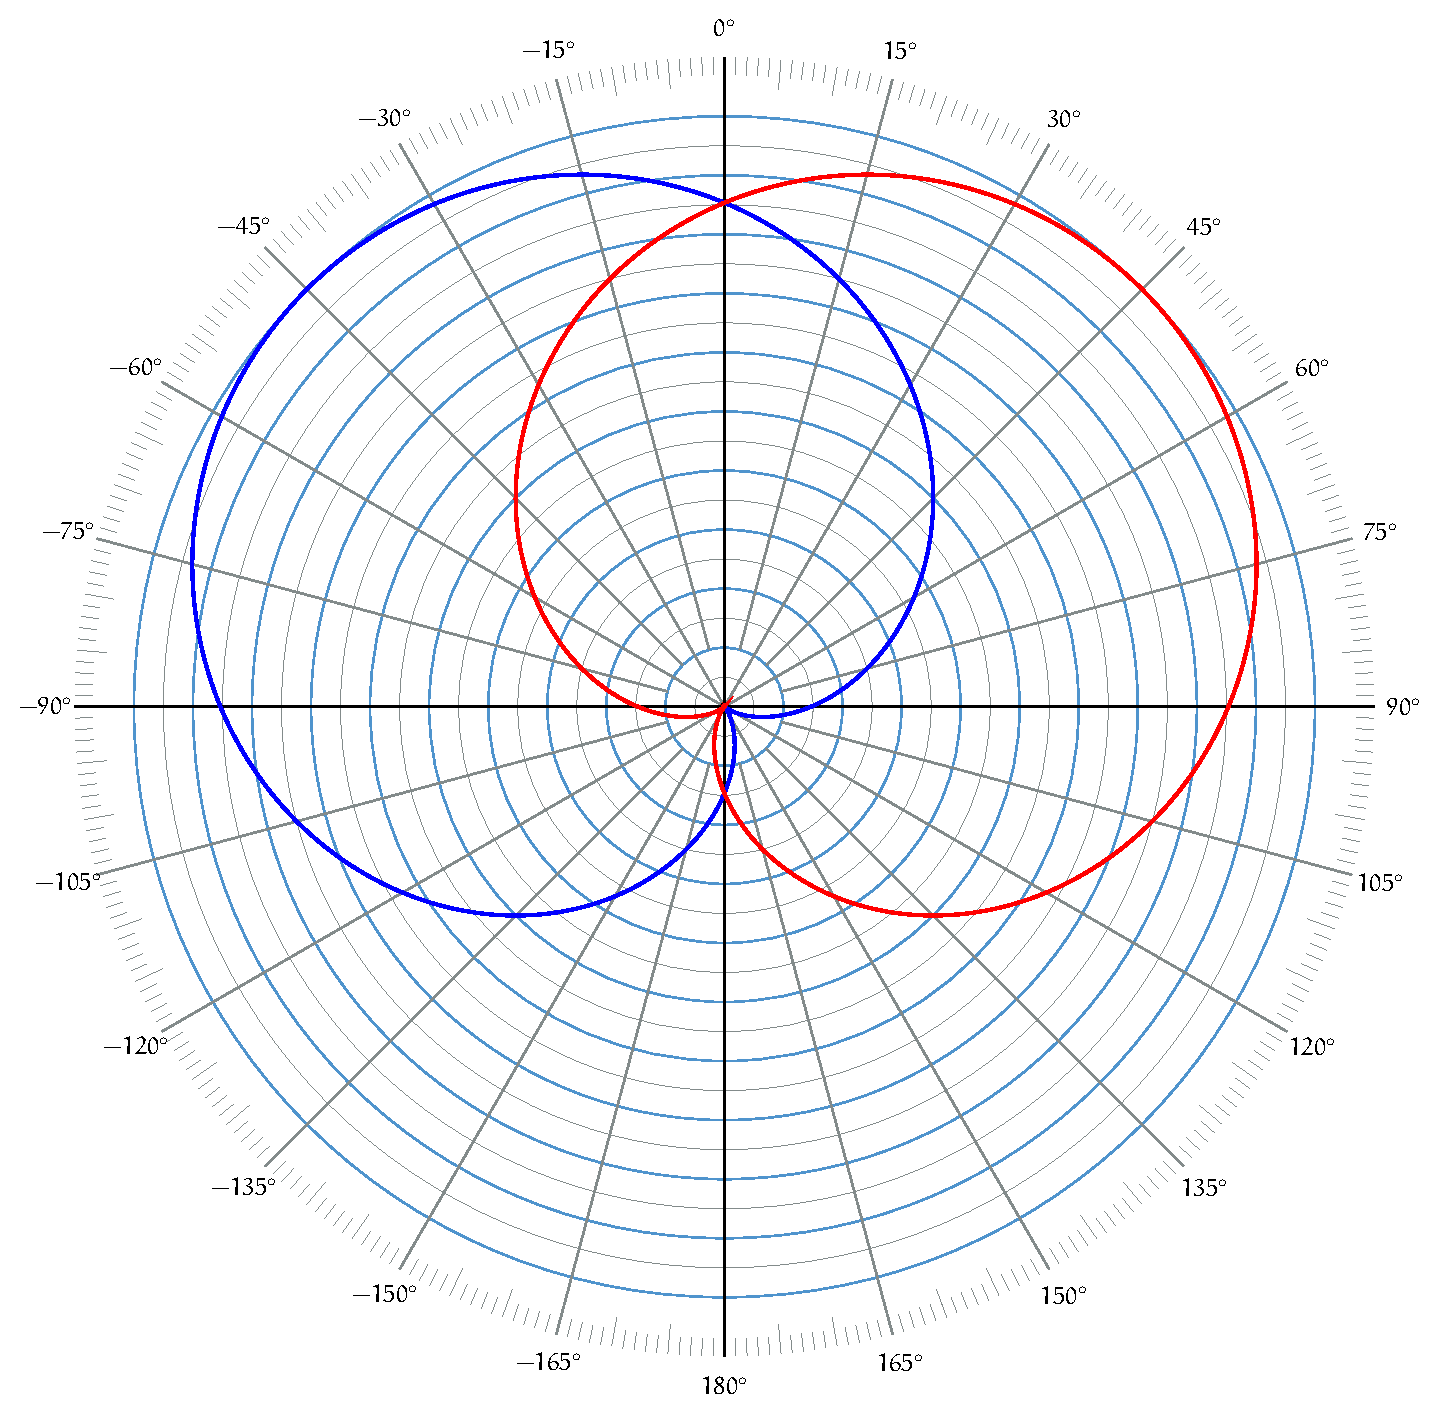
\includegraphics[width=11cm]{microphone-polar-patterns/xy90}
        \caption{XY90. Coppia stereofonica coincidente di cardioidi angolati tra loro di $90°$.}% \\ Eq: $1(x)$}
        \label{pol:xy90sp}
    \end{subfigure}%
    \\
    \begin{subfigure}[t]{0.99\textwidth}
        \centering
        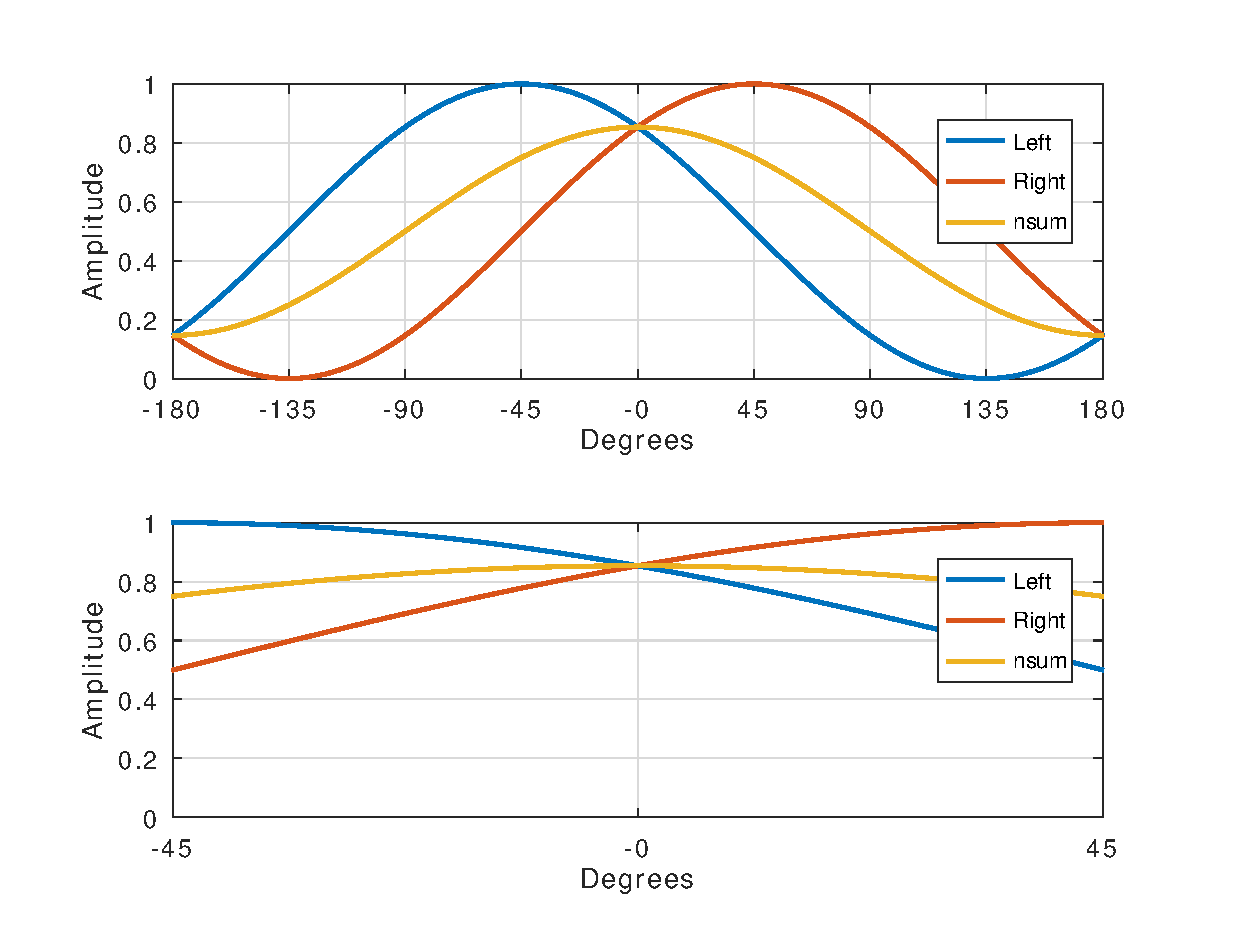
\includegraphics[width=12.5cm]{CAPITOLI/1000/IMG/xy90sub}
        \caption{Variazioni angolari di ampiezza.}% \\ Eq: $0.75(x)+0.25(x\cos\theta)$}
        \label{plot:xy90}
    \end{subfigure}
    \caption{XY90}
    \label{sp:xy90}
\end{figure*}

\clearpage

\begin{figure*}[t]
    \centering
    \begin{subfigure}[t]{0.99\textwidth}
        \centering
        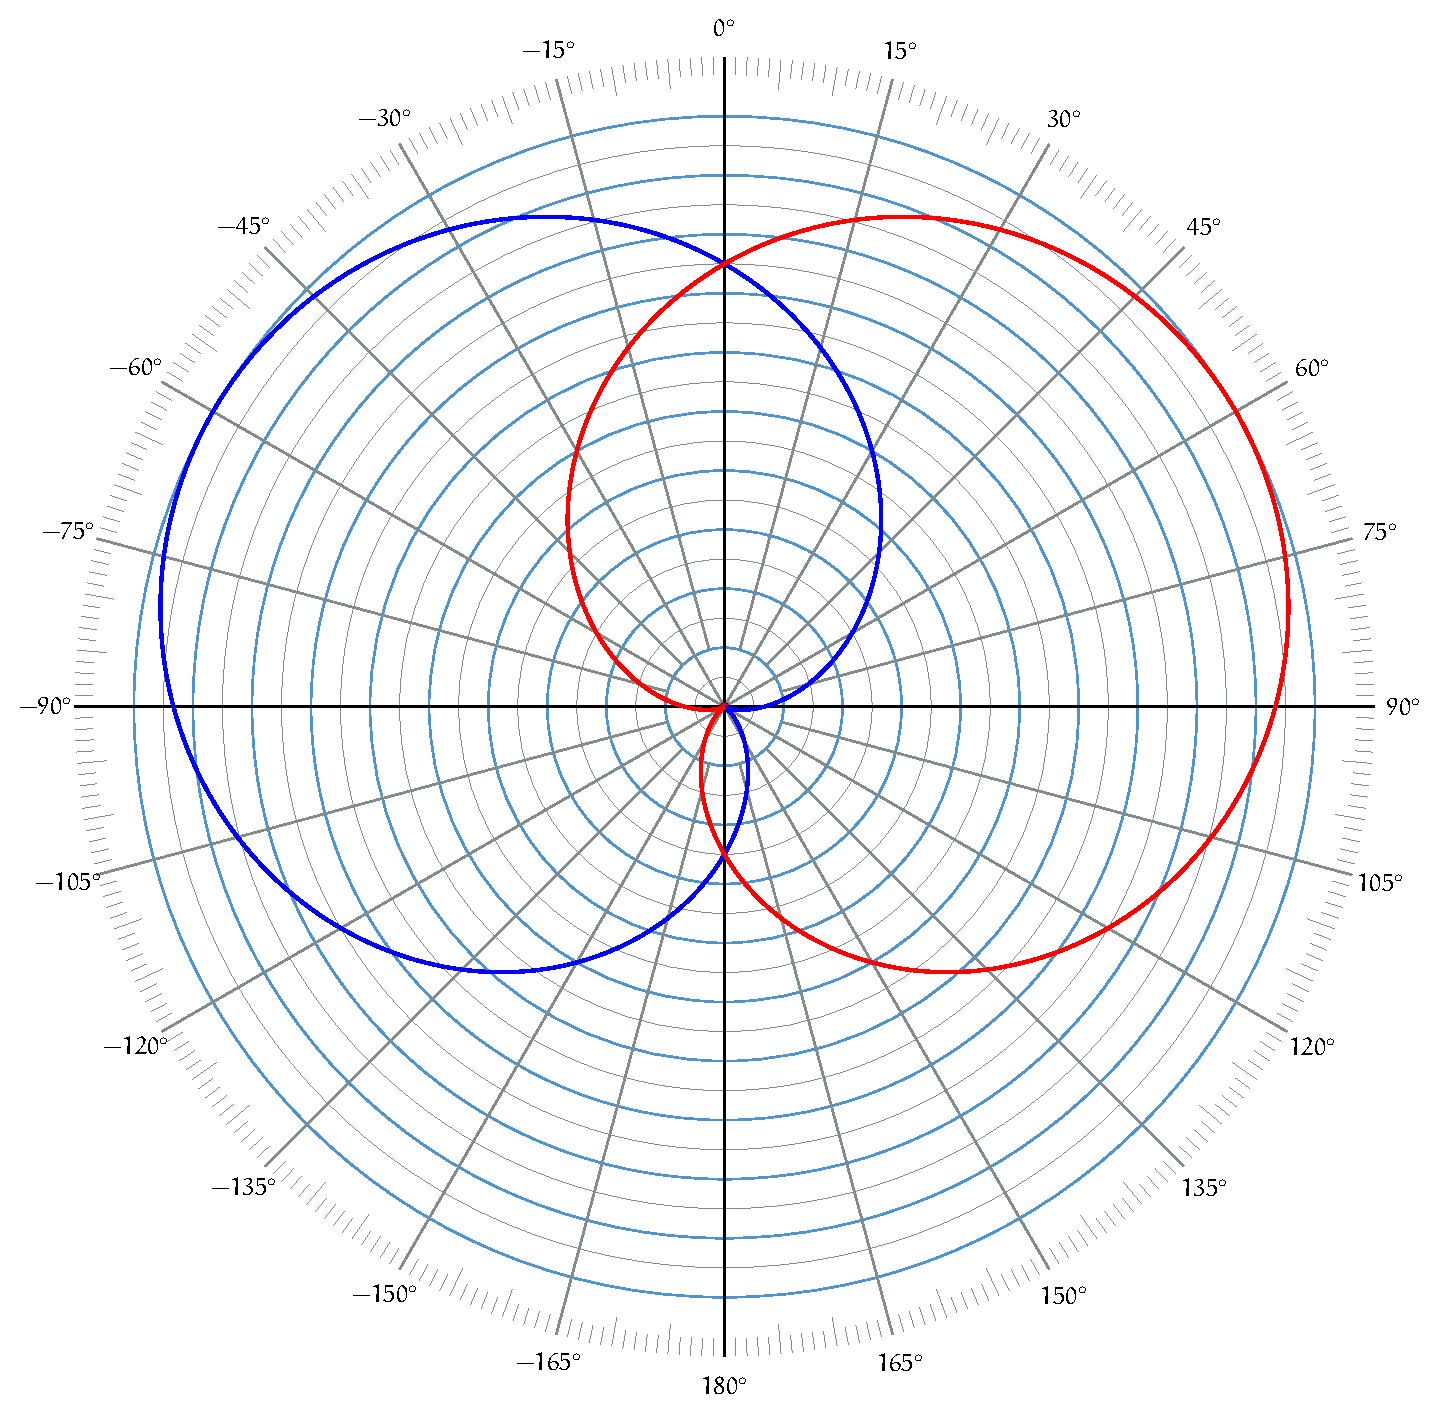
\includegraphics[width=11cm]{microphone-polar-patterns/xy120}
        \caption{XY90. Coppia stereofonica coincidente di cardioidi angolati tra loro di $120°$.}% \\ Eq: $1(x)$}
        \label{pol:xy120sp}
    \end{subfigure}%
    \\
    \begin{subfigure}[t]{0.99\textwidth}
        \centering
        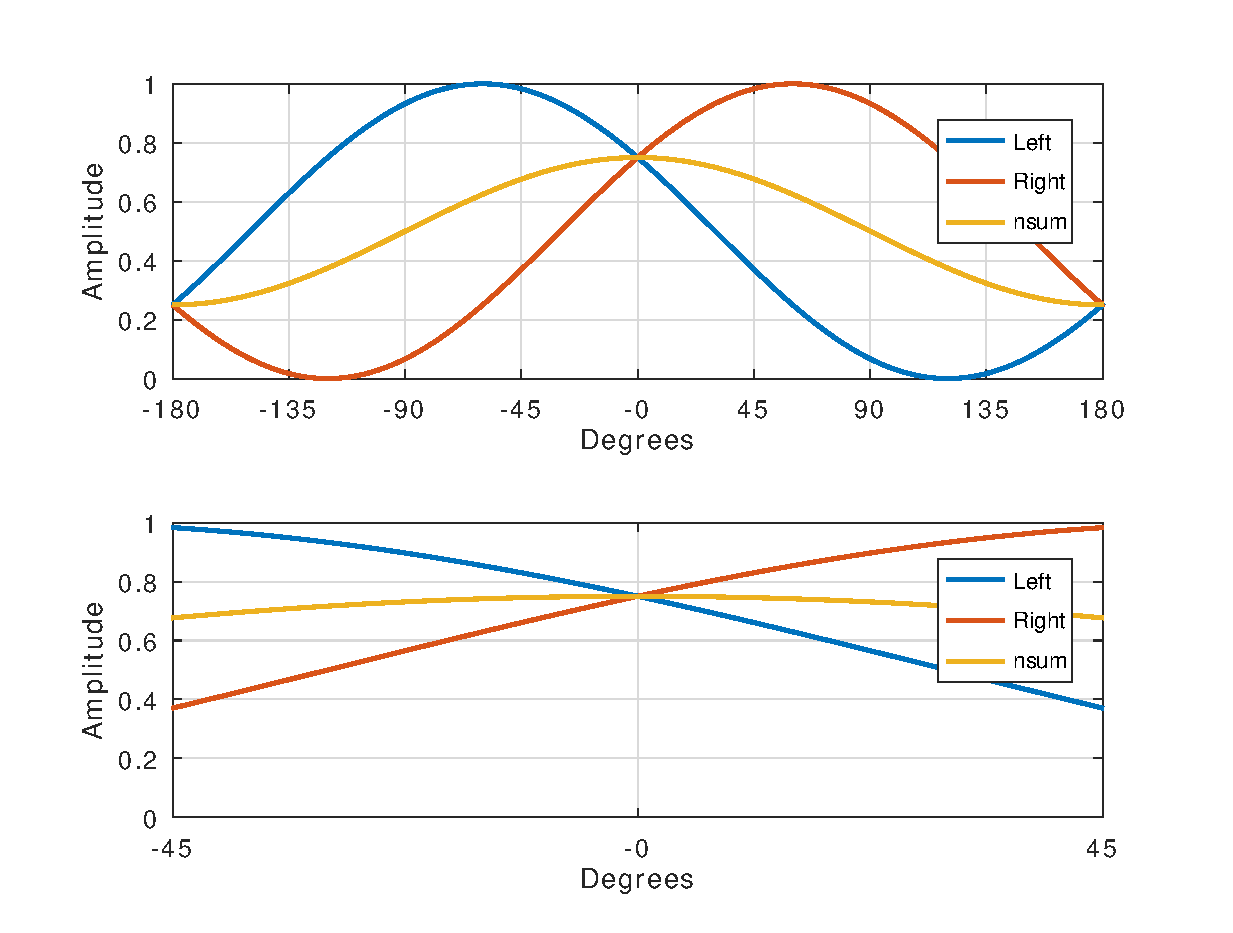
\includegraphics[width=12.5cm]{CAPITOLI/1000/IMG/xy120sub}
        \caption{Variazioni angolari di ampiezza.}% \\ Eq: $0.75(x)+0.25(x\cos\theta)$}
        \label{plot:xy120}
    \end{subfigure}
    \caption{XY120}
    \label{sp:xy120}
\end{figure*}

\clearpage

\begin{figure*}[t]
    \centering
    \begin{subfigure}[t]{0.99\textwidth}
        \centering
        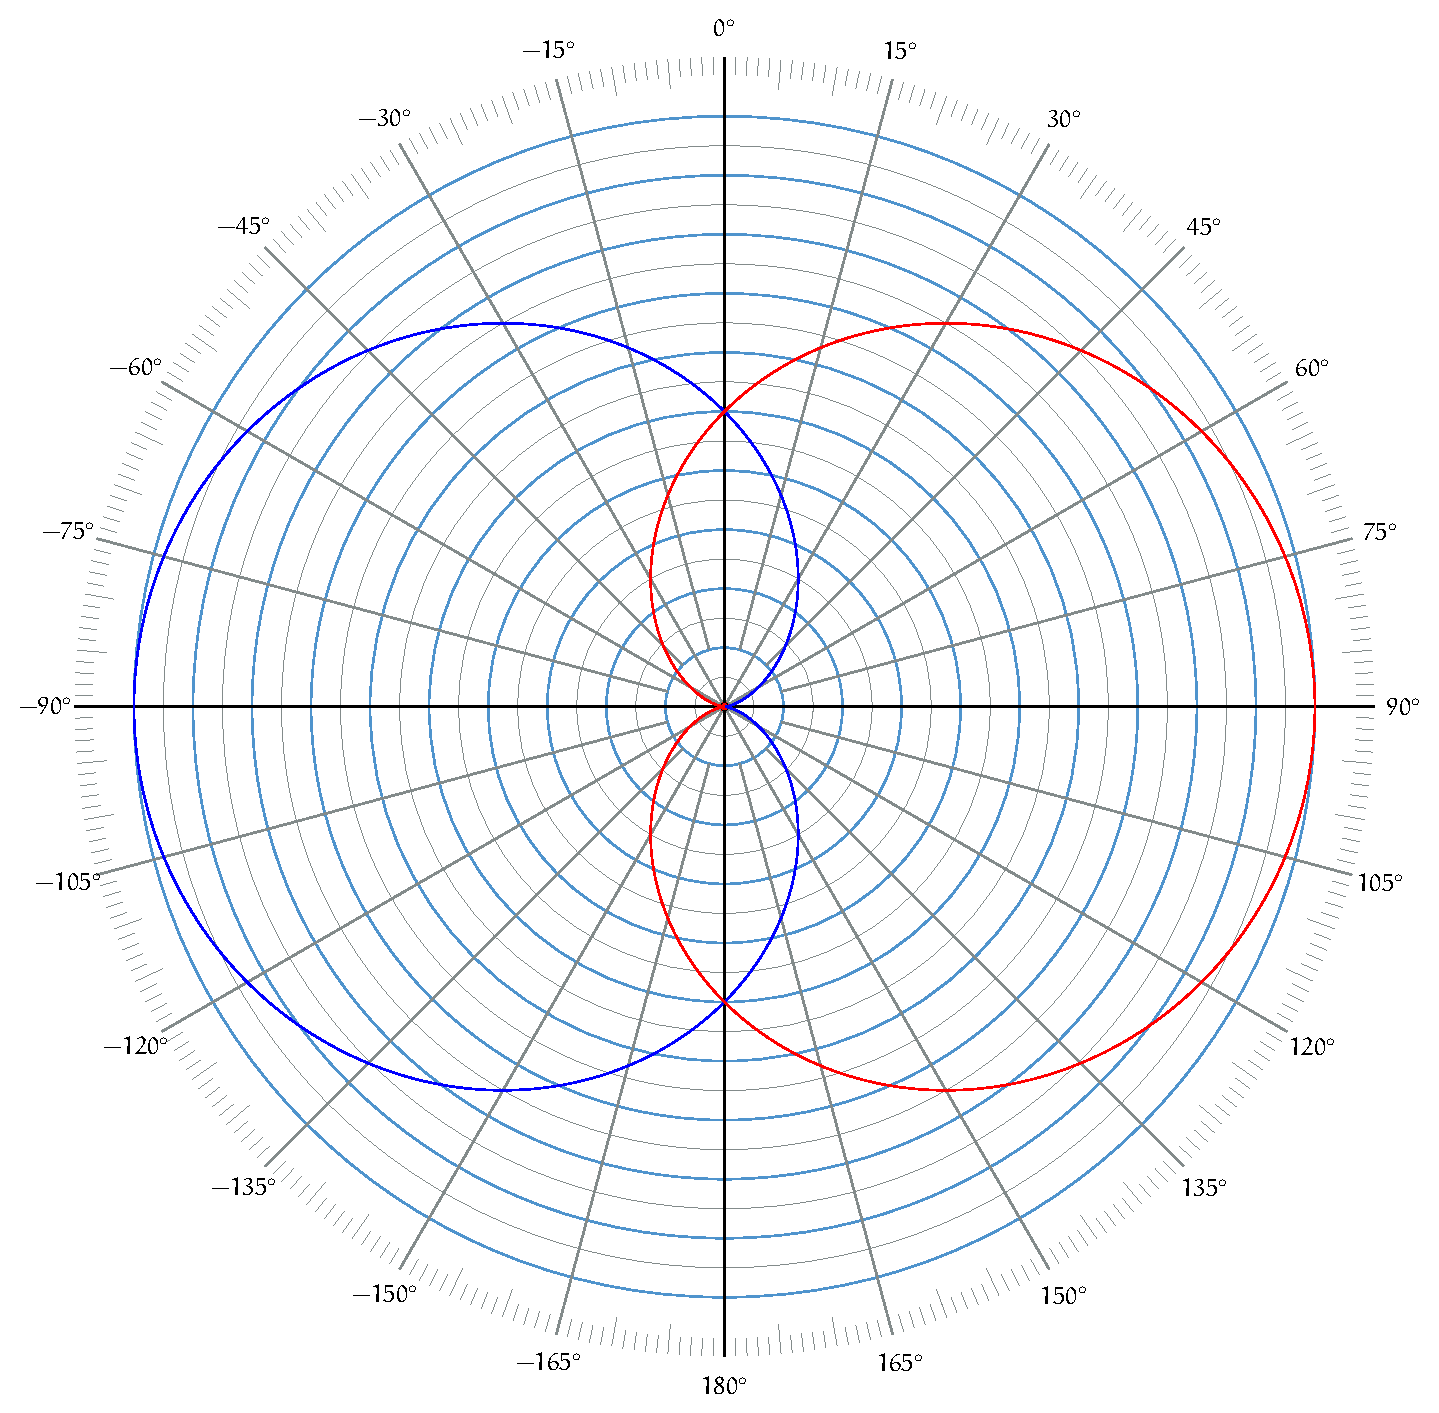
\includegraphics[width=11cm]{microphone-polar-patterns/xy180}
        \caption{XY90. Coppia stereofonica coincidente di cardioidi angolati tra loro di $180°$.}% \\ Eq: $1(x)$}
        \label{pol:xy120sp}
    \end{subfigure}%
    \\
    \begin{subfigure}[t]{0.99\textwidth}
        \centering
        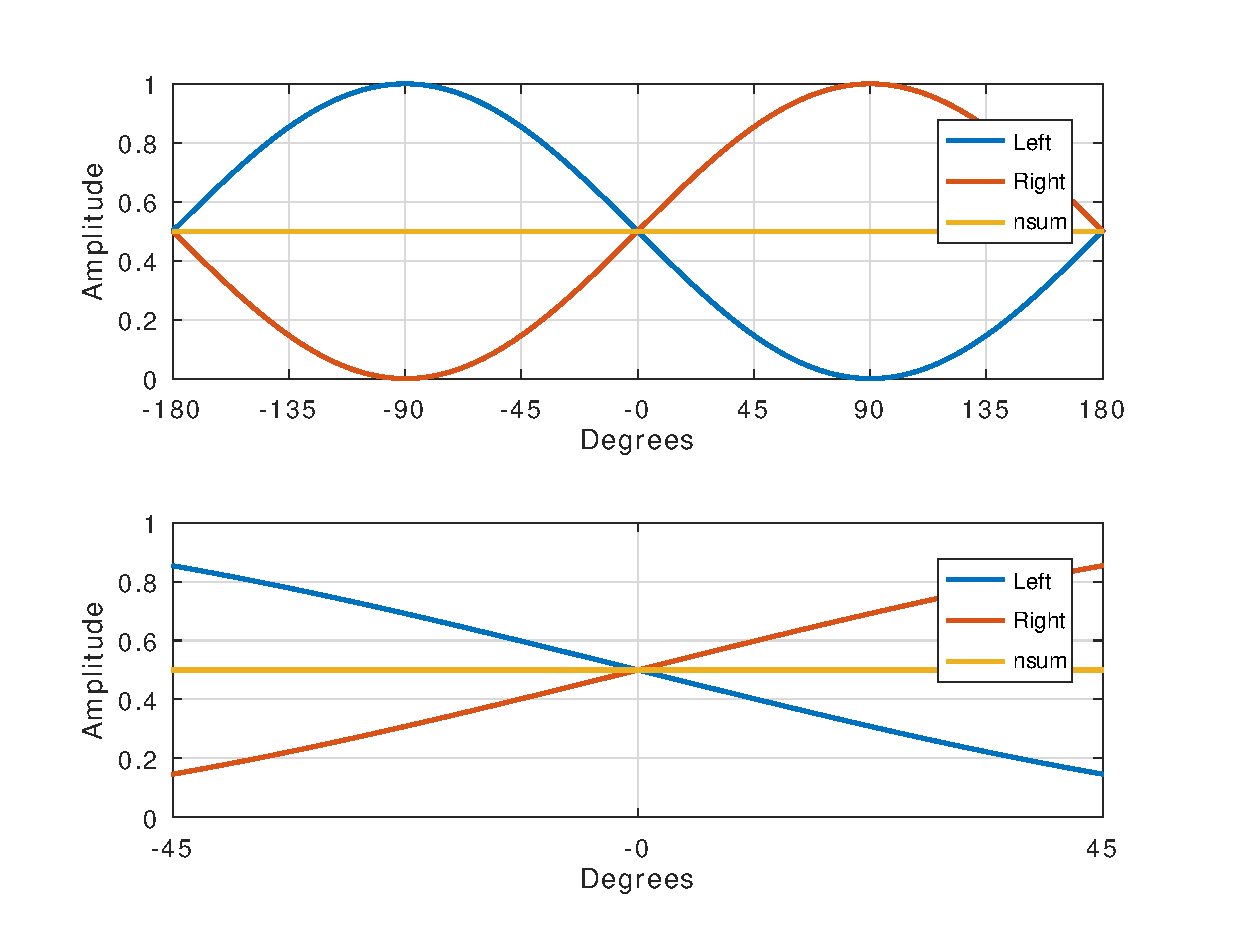
\includegraphics[width=12.5cm]{CAPITOLI/1000/IMG/xy180sub}
        \caption{Variazioni angolari di ampiezza.}% \\ Eq: $0.75(x)+0.25(x\cos\theta)$}
        \label{plot:xy180}
    \end{subfigure}
    \caption{XY180}
    \label{sp:xy180}
\end{figure*}

\clearpage

\begin{figure*}[t]
    \centering
    \begin{subfigure}[t]{0.99\textwidth}
        \centering
        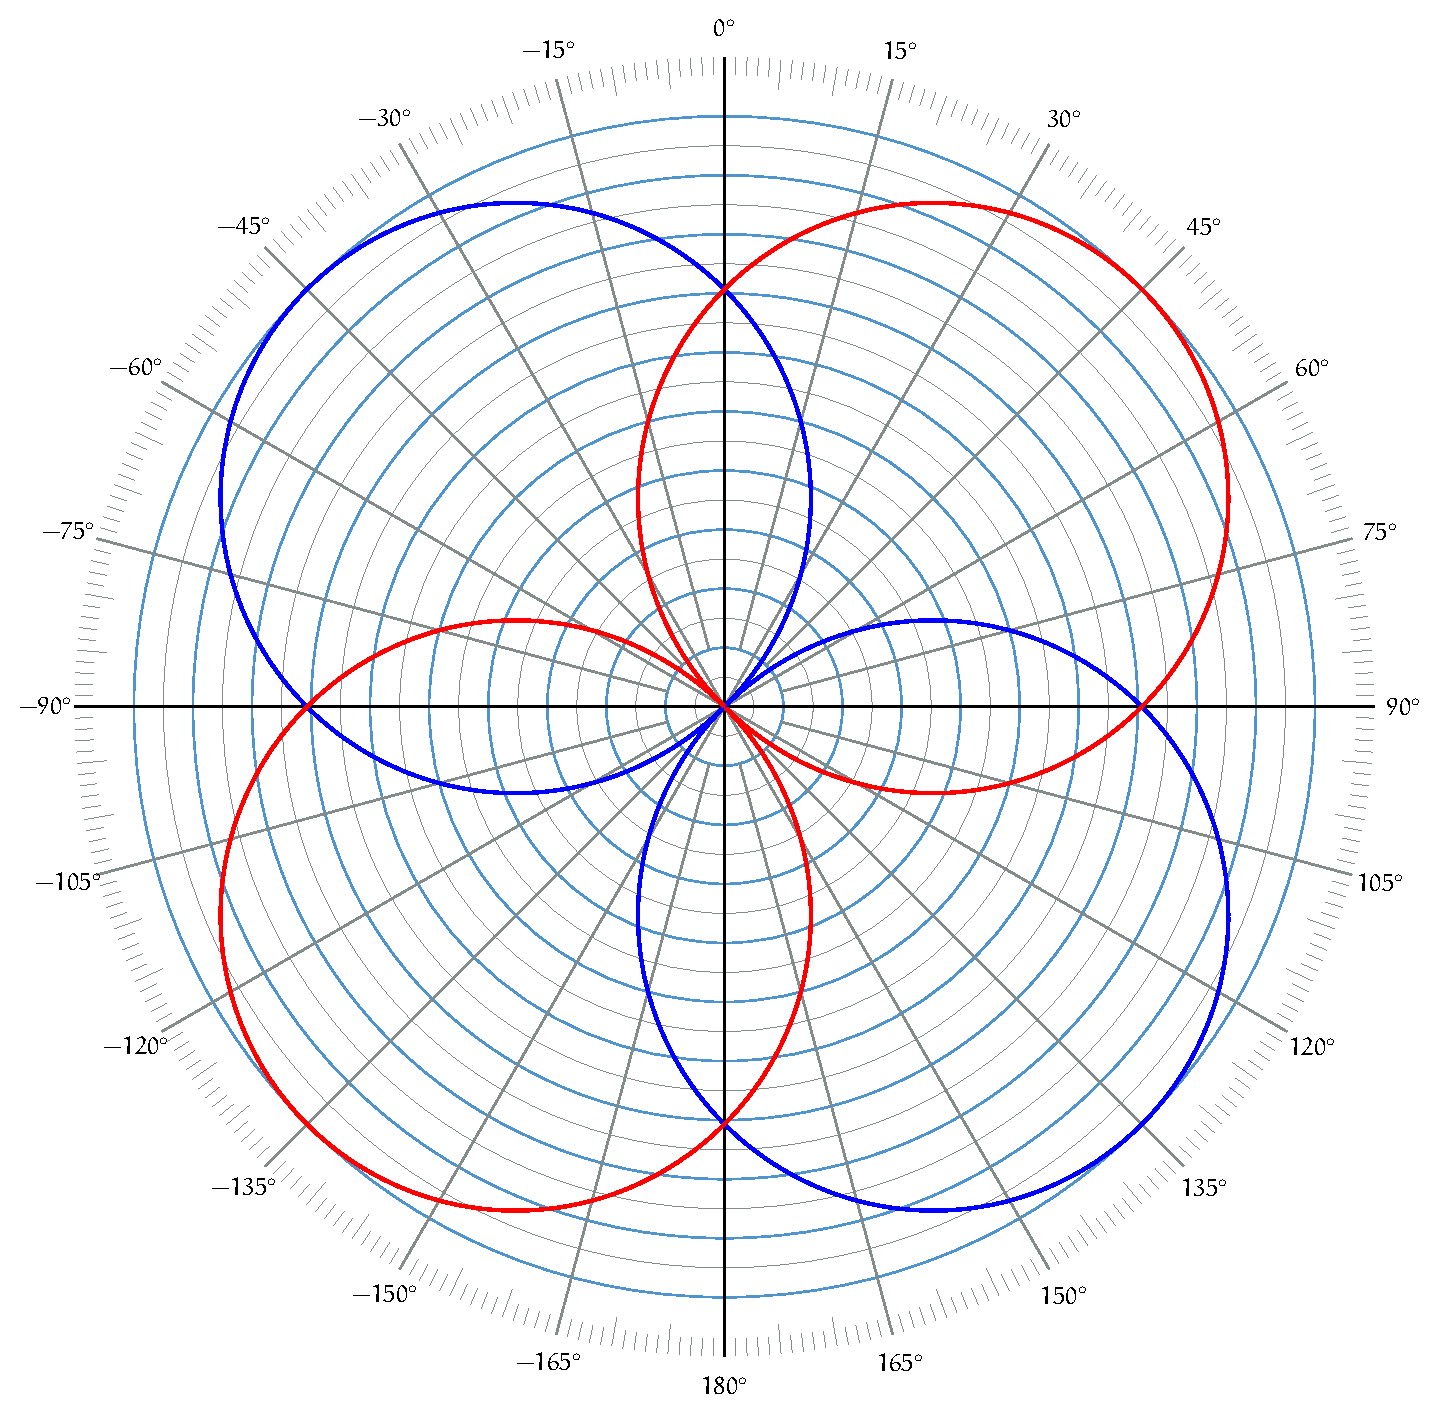
\includegraphics[width=11cm]{microphone-polar-patterns/blumlein}
        \caption{BLUMLEIN. Coppia stereofonica coincidente di figura-8 angolati tra loro di $90°$.}% \\ Eq: $1(x)$}
        \label{pol:blumleinsp}
    \end{subfigure}%
    \\
    \begin{subfigure}[t]{0.99\textwidth}
        \centering
        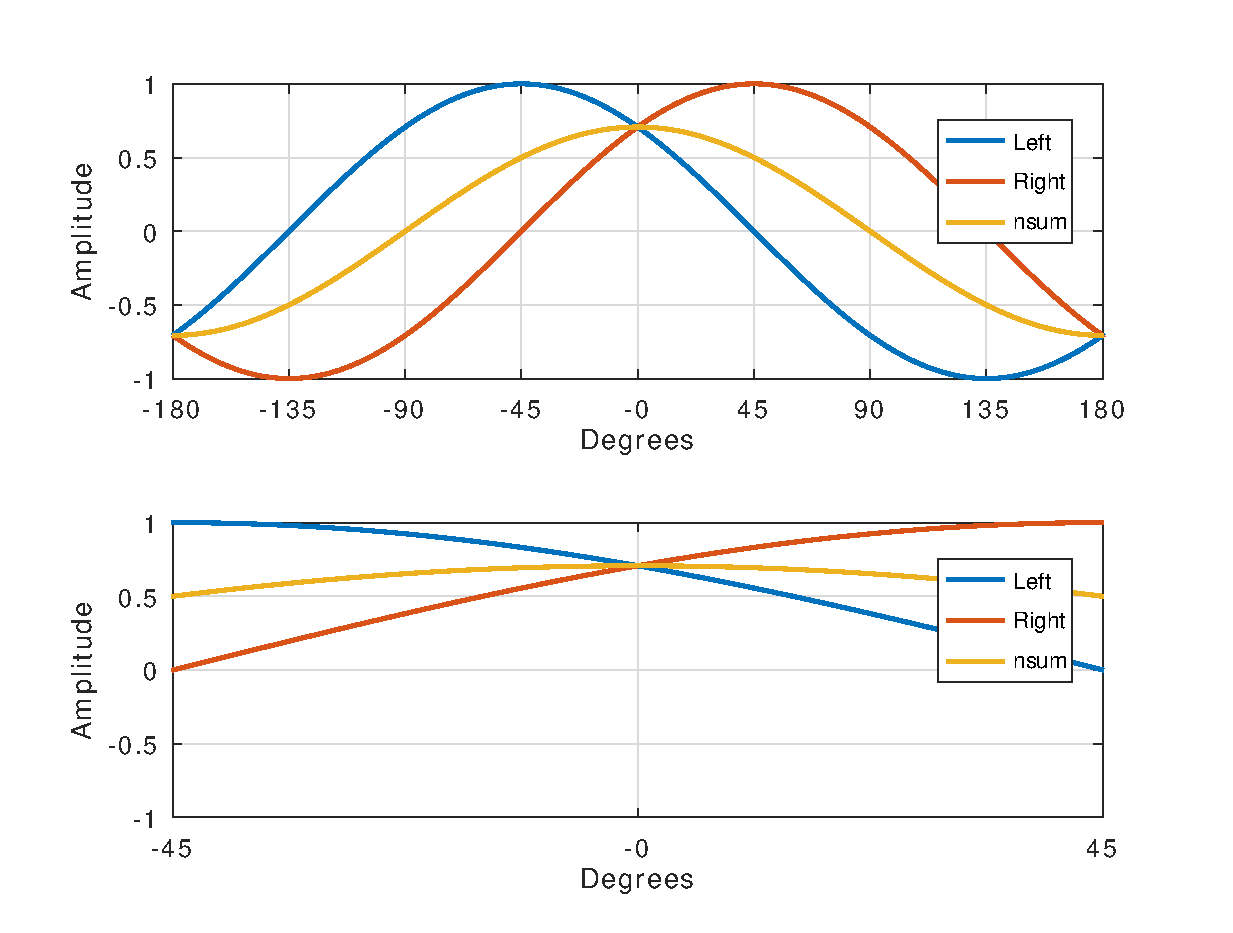
\includegraphics[width=12.5cm]{CAPITOLI/1000/IMG/blumleinsub}
        \caption{Variazioni angolari di ampiezza.}% \\ Eq: $0.75(x)+0.25(x\cos\theta)$}
        \label{plot:blumlein}
    \end{subfigure}
    \caption{BLUMLEIN}
    \label{sp:blumlein}
\end{figure*}

\clearpage

\subsection{Semi-coincidenti}

\begin{figure*}[t]
    \centering
    \begin{subfigure}[t]{0.99\textwidth}
        \centering
        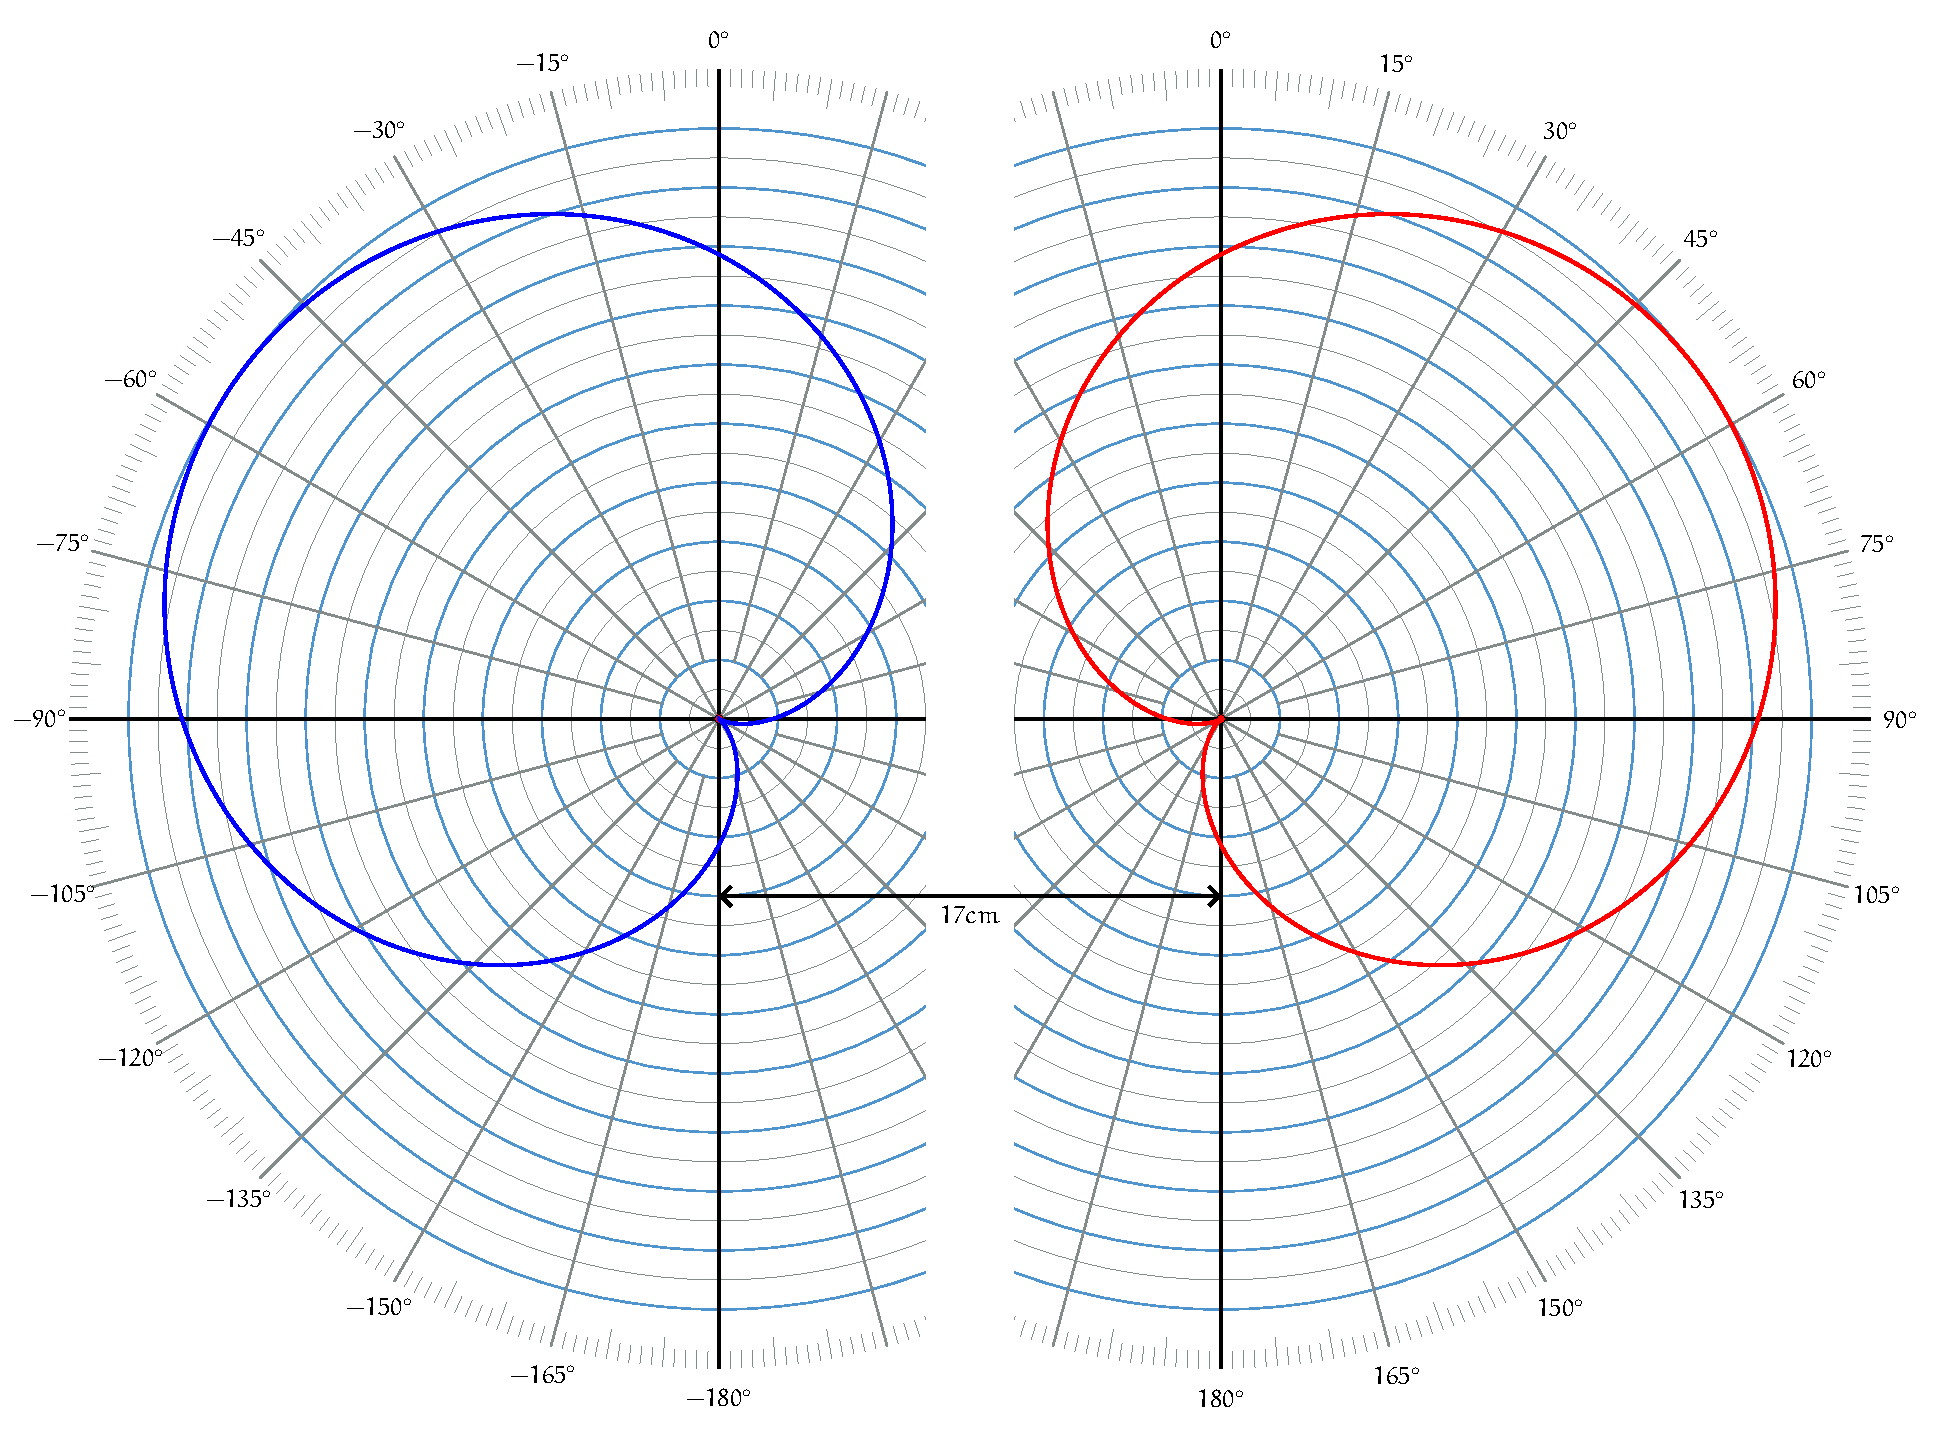
\includegraphics[width=11cm]{microphone-polar-patterns/ORTF}
        \caption{ORTF. Coppia stereofonica semi-coincidente di cardioidi angolati tra loro di $110°$ e distanti $17cm$.}% \\ Eq: $1(x)$}
        \label{pol:ortfsp}
    \end{subfigure}%
    \\
    \begin{subfigure}[t]{0.99\textwidth}
        \centering
        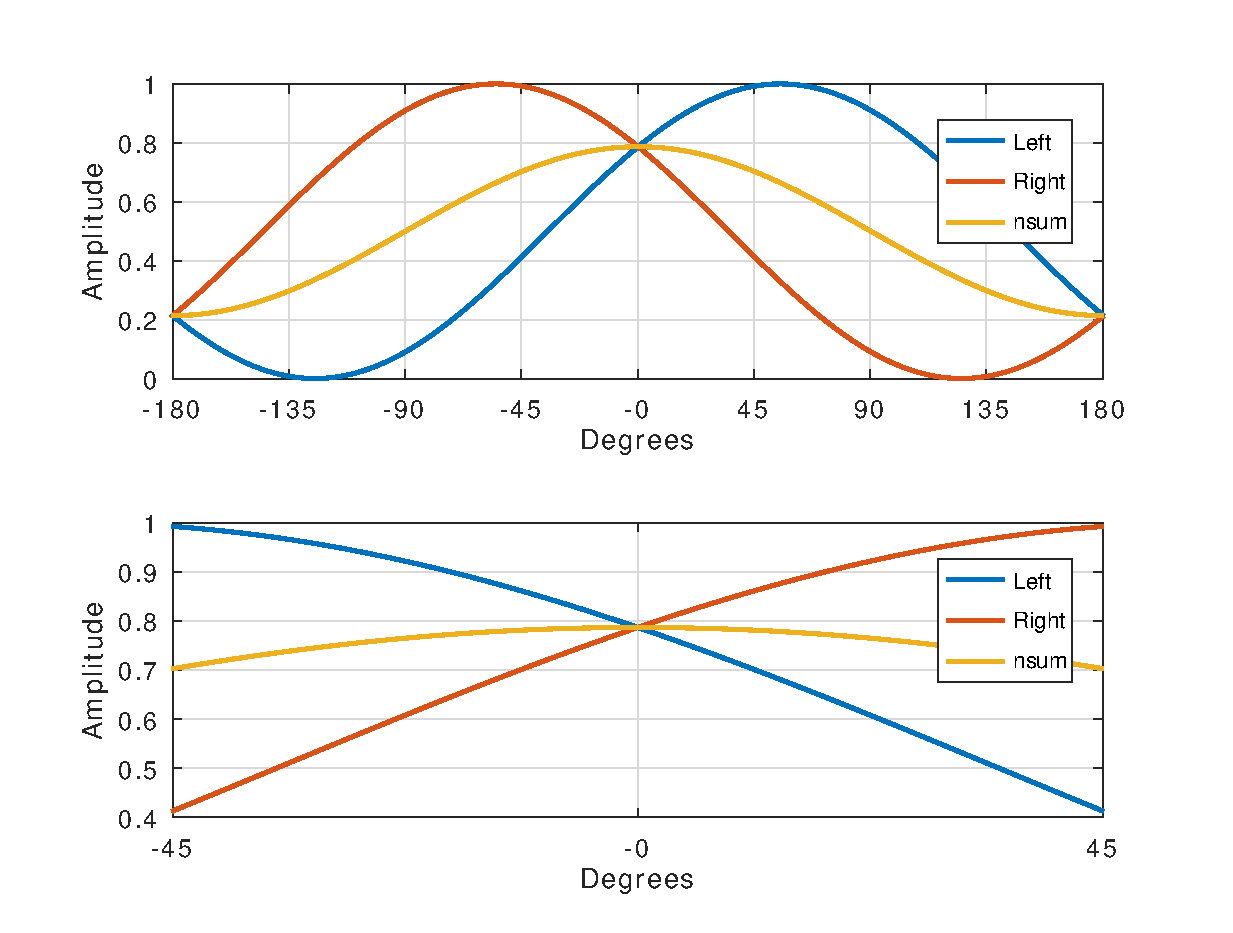
\includegraphics[width=12.5cm]{CAPITOLI/1000/IMG/ortfsub}
        \caption{Variazioni angolari di ampiezza.}% \\ Eq: $0.75(x)+0.25(x\cos\theta)$}
        \label{plot:ortf}
    \end{subfigure}
    \caption{ORTF}
    \label{sp:ortf}
\end{figure*}
